\documentclass[11pt,letterpaper]{article}

\usepackage[utf8]{inputenc}
\usepackage[spanish,es-nodecimaldot]{babel}
\usepackage{amsmath}
\usepackage{amssymb}
\usepackage{graphicx}

\usepackage{multicol}

\usepackage{tabu}

\usepackage[most]{tcolorbox}

\usepackage{mathtools}
\usepackage{tikz}
\usetikzlibrary{trees,positioning}

\usepackage[top=1in, bottom=1in, left=1in, right=1in]{geometry}


\begin{document}

\begin{titlepage}
    \centering

    {\scshape\LARGE Universidad Nacional Autónoma de México \par}

    \vspace{1cm}
    {\scshape\Large Facultad de Ciencias\par}
    \vspace{1.5cm}

    \begin{center}
        
\includegraphics[scale=.1]{../../assets/img/logo.png}
    \end{center}

    \vspace{.8 cm}

    {\LARGE Tarea semanal 06: \par}
    {\huge\bfseries Circuitos lógicos \par}

    \vspace{0.5cm}
    {\large\itshape Pablo A. Trinidad Paz\par}
    419004279

    \vfill

    Trabajo presentado como parte del curso de \textbf{Estructuras Discretas}
    impartido por la profesora \textbf{Pilar Selene Linares Arévalo}. \par
    \vspace{0.1cm}
    {\large 12 de Septiembre de 2018\par}
\end{titlepage}

\begin{enumerate}
    \item Demuestra que los siguientes circuitos son equivalentes
        \begin{center}
            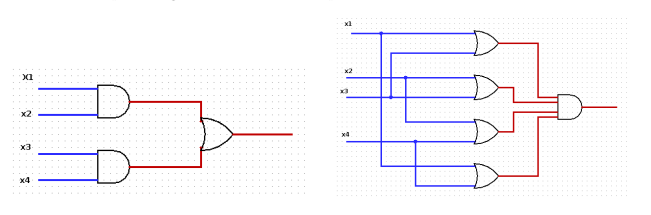
\includegraphics[scale=.5]{./assets/1.png}
        \end{center}

        \begin{equation*} \begin{split} \begin{gathered}
            (x_1 x_2) + (x_3 x_4) \equiv (x_1 + x_3) (x_2 + x_3) (x_2 + x_4) (x_1 + x_4) \\
            \text{Por distributibidad:} \\
            (x_1 + x_3) (x_2 + x_3) (x_2 + x_4) (x_1 + x_4) \equiv (x_1 + x_3) (x_2 + x_3) (x_2 + x_4) (x_1 + x_4)
        \end{gathered} \end{split} \end{equation*}

    \item Para cado uno de los siguientes incisos decide si la construcción de bloques
    propuesta es válida y óptima. Si no lo es, indica por qué y genera una válida o bien, mejórala
        \begin{enumerate}
            \begin{multicols}{3}
                \item \begin{center} 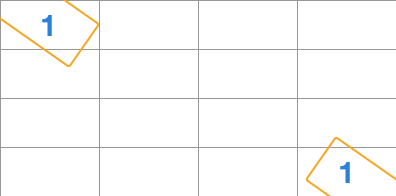
\includegraphics[scale=.3]{./assets/2a.png} \end{center}
                    Sí es válida y óptima. Es válida por la definición de adyacencia que especifica
                    que si sólo cambia el valor de una de las variables por columna y rengón, entonces
                    las celdas son adyacentes.

                \bigskip \hrule \bigskip
                \item \begin{center} 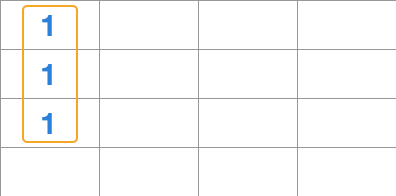
\includegraphics[scale=.3]{./assets/2b.png} \end{center}
                    No es válida porque los bloques tienen que tener $n$ elementos donde $n$ tiene
                    que se potencia de dos. En este caso 3 no es potencia de 2. La solución válida
                    y óptima sería:
                        \begin{center} 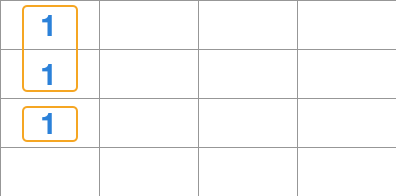
\includegraphics[scale=.3]{./assets/valid2b.png} \end{center}

                \bigskip \hrule \bigskip
                \item \begin{center} 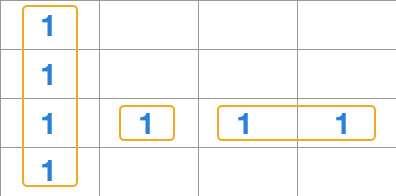
\includegraphics[scale=.3]{./assets/2c.png} \end{center}
                    Sí es válida pero no es óptima. El objetivo es crear la menor cantidad de bloques,
                    por lo que la solución óptima sería:
                        \begin{center} 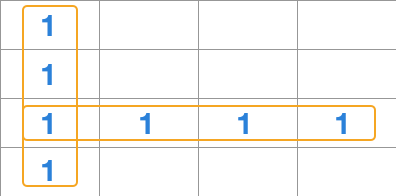
\includegraphics[scale=.3]{./assets/valid2c.png} \end{center}

                \bigskip \hrule
                \item \begin{center} 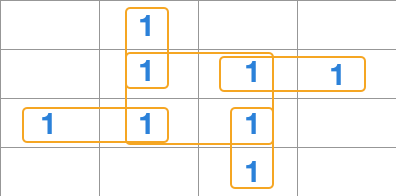
\includegraphics[scale=.3]{./assets/2d.png} \end{center}
                    Sí es válida pero no es óptima. La solución óptima sería la versión mostrada
                    en el inciso $e$, nuevamente por el objetivo de crear la menor cantidad
                    de bloques.

                \bigskip \hrule \bigskip
                \item \begin{center} 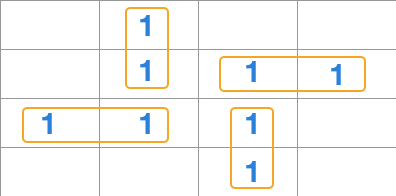
\includegraphics[scale=.3]{./assets/2e.png} \end{center}
                    Sí es válida y óptima.
            \end{multicols}
        \end{enumerate}

    \clearpage
    \item Un ventilador puede girar en dos sentidos: izquiera o derecha. En el panel de control
    se encuentran tres botones con las siguientes etiquetas: $D, I, C$, los cuales corresponden
    al \textit{giro a la derecha, giro a la izquierda y control de selección} respectivamente.
    Las señales enviadas por los botones definen el movimiento del ventilador bajo las siguientes
    condiciones:
        \begin{itemize}
            \item Si se pulsa alguno de los botones de giro, entonces el ventilador gira en el
            sentido correspondiente.
            \item Si no se presiona alguno de los botones de giro, el ventilador no gira.
            \item Si se presionan los dos botones $D$ e $I$ simultáneamente, el sentido del giro
            depende del botón de control:
                \begin{itemize}
                    \item Si se presiona $C$, el ventilador gira a la derecha.
                    \item Si no se presiona $C$, el ventilador gira a la izquierda.
                \end{itemize}
        \end{itemize}

        \begin{enumerate}
            \item Construye la tabla que representa el comportamiento del ventilado dadas
            las entradas $C, D, I$ del panel. (Las salidas $S1$ y $S2$ indican si el ventilador
            gira a la izquierda o derecha respectivamente.) \\

                \begin{center}
                    {\tabulinesep=1.2mm \begin{tabu} { c c c | c c }
                        $D$ & $I$ & $C$ & $S1$ & $S2$ \\
                        \hline
                        0 & 0 & 0       & 0 & 0 \\
                        0 & 0 & 1       & 0 & 0 \\
                        \hline
                        0 & 1 & 0       & 1 & 0 \\
                        0 & 1 & 1       & 1 & 0 \\
                        \hline
                        1 & 0 & 0       & 0 & 1 \\
                        1 & 0 & 1       & 0 & 1 \\
                        \hline
                        1 & 1 & 0       & 1 & 0 \\
                        1 & 1 & 1       & 0 & 1 \\
                    \end{tabu}}
                \end{center}
            \item Obtén las funciones booleanas para $S1$ y $S2$

                \begin{equation*} \begin{split} \begin{gathered}
                    S1(D, I, C) = \bar{D}I\bar{C} + \bar{D}IC + DI\bar{C} \\
                    S2(D, I, C) = D\bar{I}\bar{C} + D\bar{I}C + DIC
                \end{gathered} \end{split} \end{equation*}
            \item Minimiza las funciones obtenidas en $b)$ con el método de tu preferencia.
                \begin{center}
                    Karnaugh para $S1$ \\
                    {\tabulinesep=1.2mm \begin{tabu} { c | c c c c }
                        & $DI$ & $D\bar{I}$ & $\bar{D}\bar{I}$ & $\bar{D}I$ \\
                        \hline
                        $C$ &  &   &   & 1 \\
                        $\bar{C}$ & 1 &   &   & 1 \\
                    \end{tabu}}
                \end{center}
                \begin{equation*} \begin{split} \begin{gathered}
                    \tcboxmath{S1(D, I, C) = I + \bar{C}I}
                \end{gathered} \end{split} \end{equation*}
                \clearpage
                \begin{center}
                    Karnaugh para $S2$ \\
                    {\tabulinesep=1.2mm \begin{tabu} { c | c c c c }
                        & $DI$ & $D\bar{I}$ & $\bar{D}\bar{I}$ & $\bar{D}I$ \\
                        \hline
                        $C$ & 1 & 1 &  & \\
                        $\bar{C}$ &  & 1 &   &  \\
                    \end{tabu}}
                \end{center}
                \begin{equation*} \begin{split} \begin{gathered}
                    \tcboxmath{S1(D, I, C) = CD + D}
                \end{gathered} \end{split} \end{equation*}
        \end{enumerate}

\end{enumerate}

\end{document}
